\chapter{Objectifs, definitions, contraintes}
\section{Introduction aux réseaux wifi}

\begin{figure}
   \centering
   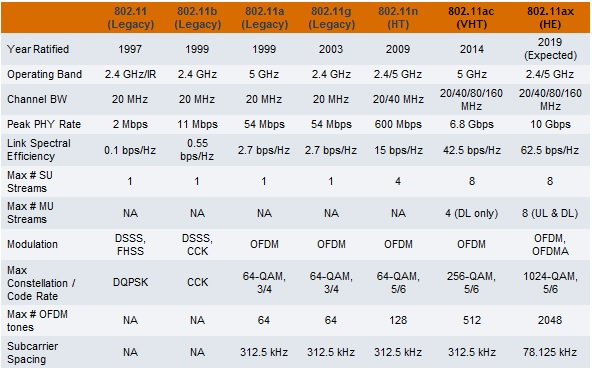
\includegraphics[width=0.8\textwidth,natwidth=488,natheight=513]{images/diffwifi.jpg}
   \caption{Différences entre les normes wifi IEEE 802.11}
\end{figure}
Le wifi, abréviation de wireless fidelity, est un ensemble de protocoles permettant la communication sans fil entre deux
appareils en utilisant des ondes radios. La standardisation de cette norme à été initié l'IEEE\footnote{Institute of Electrical and Electronics Engineers}
en 1990. Cela à aboutit, en 1997, au standart IEEE 802.11 définissant les réseaux locaux sans fils.\cite{WFintro}. La norme
d'origine prévoyait l'utilisation d'ondes radios dans la bande de fréquences libre entre 2401 et 2495 MHz\cite{WFband}
,courrament appelée bande à 2,4 GHz, ou par infra rouges.
Cependant, pour suivre l'évolution des technologies, le standart IEEE 802.11 s'est enrichi afin d'augmenter le débit et
d'utiliser la bande de fréqences libre entre 5170 et 5710 MHz.
Les standarts IEEE 802.11a et IEEE 802.11b à donc été définit en 1999, le standart 802.11g et 2003 et le standart 802.11n
en 2009. La figure 1.1 montre les principales différences entre les normes wifi cités plus haut.\cite{WFevol}

Depuis sa création, la norme IEEE 802.11 définit 14 cannaux dans la bande 2,4 GHz. Chaque canal à une largeur de 22 MHz et 
l'écart entre les centres de deux canaux successifs est de 5 MHz\footnote{Sauf les centres des cannaux 13 et 14 qui sont espacé
de 12 MHz}. Il en résulte donc un fort recouvrement entre les différents cannaux comme le montre la figure 1.2.

\begin{figure}
   \centering
   
\includegraphics[width=0.8\textwidth,natwidth=610,natheight=642]{images/cannaux.png}
   \caption{Répartition des cannaux dans la bande 2,4 GHz}
\end{figure}

Un réseau wifi est un réseau local découpé en ``cellules'' appelée BSS\footnote{Basic Service Set}. Deux appareils
doivent se trouver dans le même BSS pour communiquer entre eux. Il existe deux modes de BSS : Le mode Infrastructure et le
mode ad-hoc\cite{WFfunc2}. La pluspart des réseaux wifi de particuliers ou d'entreprises sont des réseaux en mode Infrastructure.

Le mode infrastructure se caractérise par le fait que chaque BSS posséde une station de base, appelé
aussi point d'accés, et que toutes les communications passent nécessairement par le point d'accés de la BSS, et ce même si 
l'émeteur et le récepteur du message se trouvent dans le même BSS. Un point d'accés peut être relié par un réseau cablé à
un ou plusieurs autres points d'accés, étendant ainsi le LAN\footnote{Local Area Network, ou Réseau local}
\cite{WFfunc},ou à un routeur pour accéder à un réseau WAN\footnote{Wide Area Network, ou Réseau étendu}.
Le mode ad-hoc, au contraire, est un mode ``d'égal à égal''. Deux entités au sein du même BSS peuvent communiquer directement.


Comme le montre la figure 1.3\cite{WFhead}, le premier champ de l'en tête wifi est le FCF\footnote{Frame Control Field, ou Champ
de contrôle de trame}, permettant d'identifier les trames en fonction de leur rôle. Ainsi, les trames peuvent être de trois types,
identifiées par les deux bits en position 3 et 4 du FCF : Management, controle ou donées.\cite{WFfcf}. Les 4 bits suivants
identifient le sous type.

Les Beacons frames sont des trames de management particuliéres qui permettent à un point d'accés de déclarer sa présence aux
appareils à proximité. Ils transportent différentes informations comme le SSID\footnote{Service Set IDentifier} du réseau,
qui est une chaîne de 2 à 32 charactéres, un timestamp permettant de se symchroniser, le canal sur lequel il émet, 
et d'autres informations.\cite{WFfunc2}.
\begin{figure}
   \centering
   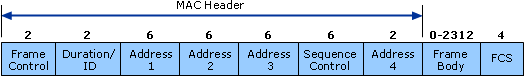
\includegraphics[width=0.8\textwidth,natwidth=488,natheight=513]{images/header_wifi.png}
   \caption{Format des trames 802.11}
\end{figure}

\section{La norme 802.11s}
\section{Adressage et routage}